\chapter{การติดตั้งเครื่องมือที่ใช้พัฒนาโปรแกรม}
การติดตั้งเครื่องมือที่ใช้ในการพัฒนาแอปพลิเคชันค้นหายาเพื่อคุณ มีโปรแกรมที่จำเป็นในการพัฒนาระบบดังต่อไปนี้
\begin{itemize}[label={--}]
	\item การติดตั้ง Node.js
    \item การติดตั้ง Ionic Framwork
    \item การติดตั้ง OpenCV
\end{itemize}

\section{การติดตั้ง Node.js}
    1) สามารถดาวน์โหลด Node.js ได้ที่ https://nodejs.org/en/download/ ดังแสดงในภาพที่ \ref{Fig:nodeInstall1}
      \begin{figure}[H]
          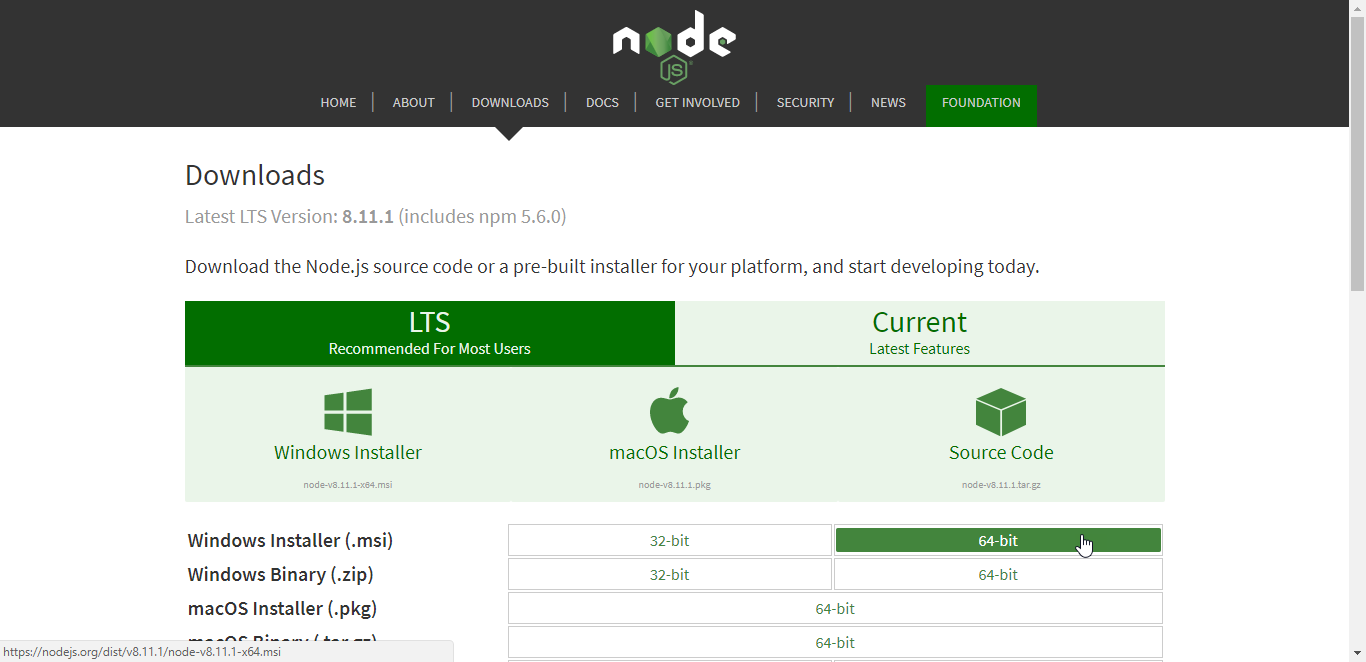
\includegraphics[width=\columnwidth]{Figures/7/1}
          \caption{หน้าเว็บดาวน์โหลด Node.js}
          \label{Fig:nodeInstall1}
      \end{figure}
      
    2) เปิดไฟล์ติดตั้ง ชื่อ node-v8.11.1-x64.msi เพื่อติดตั้ง ดังแสดงในภาพที่ \ref{Fig:nodeInstall2}
      \begin{figure}[H]
          
\includegraphics[width=\columnwidth]{Figures/7/2}
          \caption{ไฟล์ติดตั้งสำหรับติดตั้ง Node.js}
          \label{Fig:nodeInstall2}
      \end{figure}

    3) แสดงหน้าต่างตอนรับของ Node.js ให้กด Next ดังแสดงในภาพที่ \ref{Fig:nodeInstall3}
      \begin{figure}[H]
            \centering
            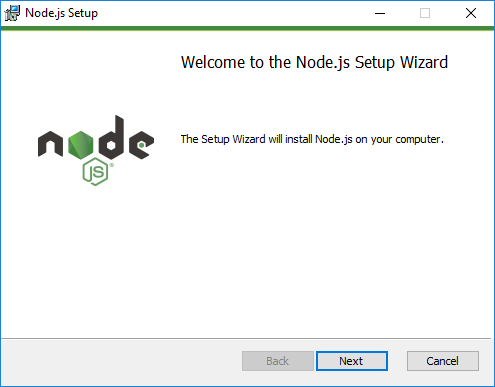
\includegraphics[width=10cm]{Figures/7/3}
            \caption{หน้าต่างตอนรับของ Node.js}
            \label{Fig:nodeInstall3}
      \end{figure}

    4) แสดงหน้าต่างข้อตกลงในการใช้ Node.js ให้เลือกช่อง I accept the terms in the License Agreement และกด Next ดังแสดงในภาพที่ \ref{Fig:nodeInstall4}
      \begin{figure}[H]
            \centering
            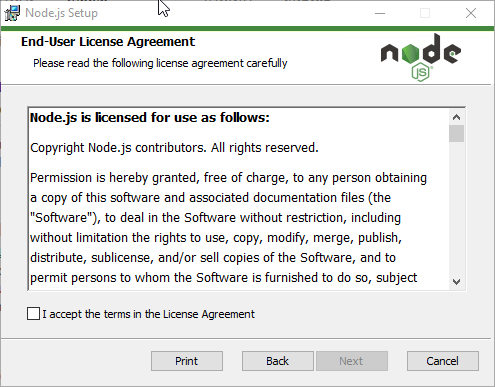
\includegraphics[width=10cm]{Figures/7/4}
            \caption{หน้าต่างข้อตกลงในการใช้ Node.js}
            \label{Fig:nodeInstall4}
      \end{figure}

    5) แสดงหน้าต่างเลือกโฟลเดอร์ที่จะทำการติดตั้ง ดังแสดงในภาพที่ \ref{Fig:nodeInstall5}
      \begin{figure}[H]
            \centering
            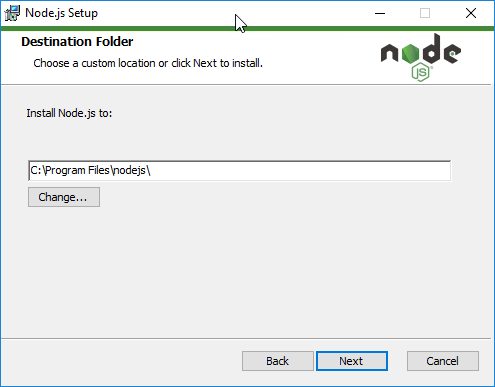
\includegraphics[width=10cm]{Figures/7/5}
            \caption{หน้าต่างเลือกโฟลเดอร์ที่จะทำการติดตั้ง Node.js}
            \label{Fig:nodeInstall5}
      \end{figure}

    6) แสดงหน้าต่างสำหรับติดตั้ง Node.js ให้กด Install เพื่อทำงานติดตั้ง ดังแสดงในภาพที่ \ref{Fig:nodeInstall6}
        \begin{figure}[H]
            \centering
            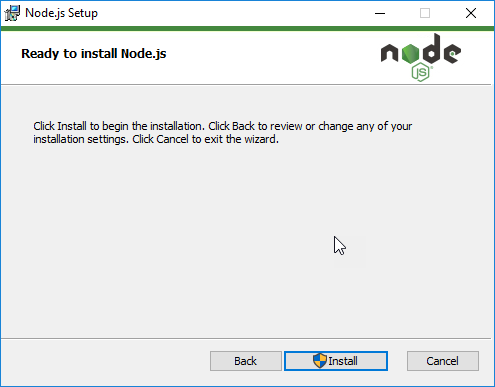
\includegraphics[width=10cm]{Figures/7/6}
            \caption{หน้าต่างติดตั้ง Node.js}
            \label{Fig:nodeInstall6}
        \end{figure}

\section{การติดตั้ง Ionic Framwork}

    การติดตั้ง Ionic Framwork สามารถทำผ่านคำสั่ง command line ได้ ดังแสดงในภาพที่ \ref{Fig:ionicInstall}
    \begin{figure}[H]
		{\setstretch{1.0}\begin{lstlisting}[numbers=none]
sudo npm  install–  g  cordova  
sudo npm  install–  g  ionic                
		\end{lstlisting}}
		\caption{คำสั่งสำหรับติดตั้ง ionic framework}
		\label{Fig:ionicInstall}
    \end{figure}
    
\section{การติดตั้ง OpenCV}
    1) สามารถดาวน์โหลด OpenCV ได้ที่ \url{https://opencv.org/releases.html} ดังแสดงในภาพที่ \ref{Fig:opencvInstall1}
      \begin{figure}[H]
          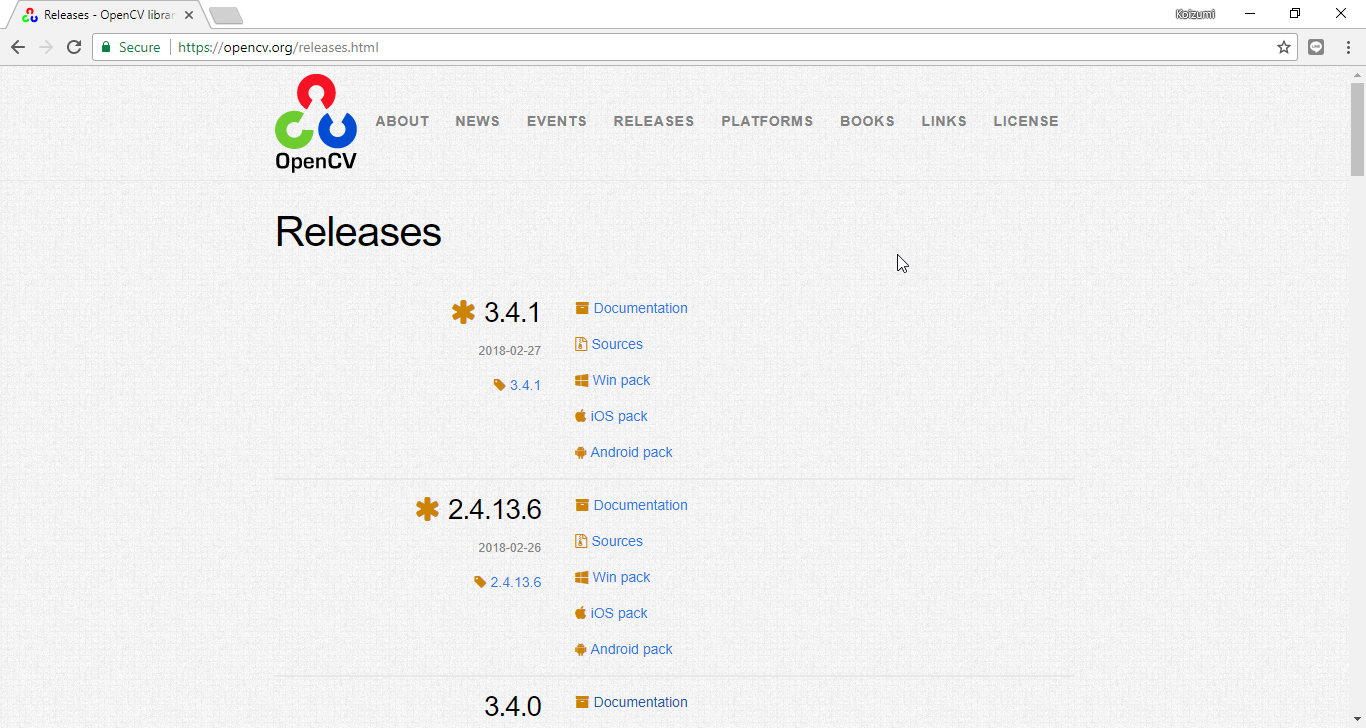
\includegraphics[width=\columnwidth]{Figures/7/7}
          \caption{หน้าเว็บสำหรับดาวน์โหลด OpenCV}
          \label{Fig:opencvInstall1}
      \end{figure}

    2) เปิดไฟล์สำหรับติดตั้ง OpenCV ดังแสดงในภาพที่ \ref{Fig:opencvInstall2}
      \begin{figure}[H]
            \centering
          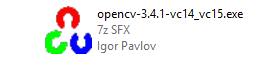
\includegraphics[width=8cm]{Figures/7/8}
          \caption{ไฟล์ติดตั้ง OpenCV}
          \label{Fig:opencvInstall2}
      \end{figure}

    3) เลือกโปรเดอร์ที่ต้องการตั้งติดและกด Extract ดังแสดงในภาพที่ \ref{Fig:opencvInstall3}
      \begin{figure}[H]
        \centering
          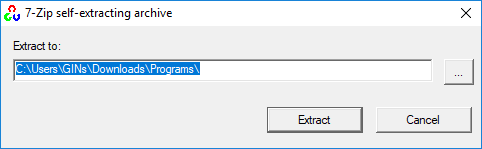
\includegraphics[width=\columnwidth]{Figures/7/9}
          \caption{เลือกโฟรเดอร์สำหรับติดตั้ง OpenCV}
          \label{Fig:opencvInstall3}
      \end{figure}

    4) เปิด This PC ขึ้นมาและคลิกขวาที่ This PC เพื่อเข้าไปที่หน้า System Properties ดังแสดงในภาพที่ \ref{Fig:opencvInstall4}
      \begin{figure}[H]
        \centering
          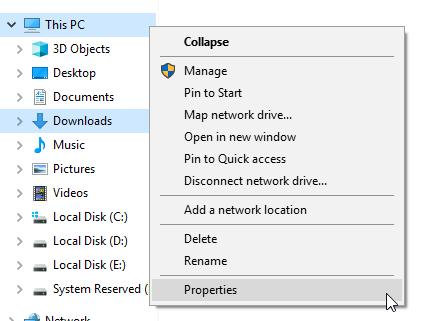
\includegraphics[width=10cm]{Figures/7/10}
          \caption{เปิด properties ของ This PC}
          \label{Fig:opencvInstall4}
      \end{figure}

    5) เลือก Advanced system setting ดังแสดงในภาพที่ \ref{Fig:opencvInstall5}
        \begin{figure}[H]
            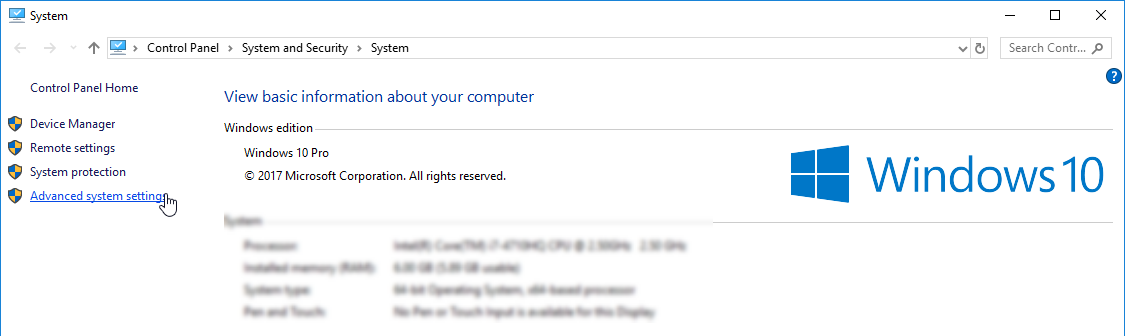
\includegraphics[width=\columnwidth]{Figures/7/11}
            \caption{หน้าต่างของ System}
            \label{Fig:opencvInstall5}
        \end{figure}

    6) เลือก Enviroment Variables ดังแสดงในภาพที่ \ref{Fig:opencvInstall6}
        \begin{figure}[H]
            \centering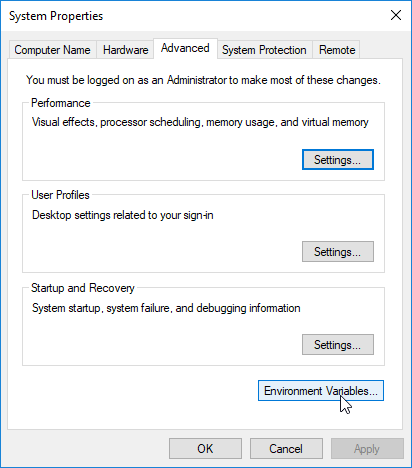
\includegraphics[width=10cm]{Figures/7/12}
            \caption{หน้าต่าง System Properties}
            \label{Fig:opencvInstall6}
        \end{figure}

    7) ทำการสร้างตัวแปร {OPENCV\_BIN\_DIR}, {OPENCV\_DIR}, {OPENCV\_INCLUDE\_DIR}, {OPENCV\_LIB\_DIR} 
    และกำหนดค่าของตัวแปร และกด OK ดังแสดงในภาพที่ \ref{Fig:opencvInstall7}
    \begin{figure}[H]
        \centering
        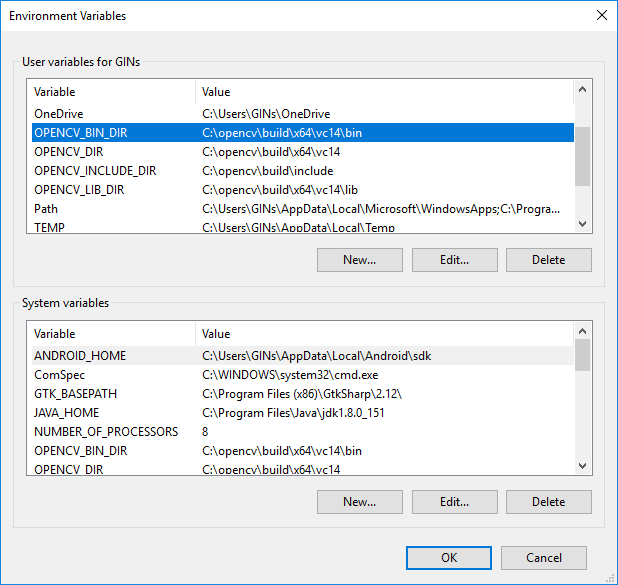
\includegraphics[width=10cm]{Figures/7/13}
        \caption{หน้าต่าง Evnironment Variables}
        \label{Fig:opencvInstall7}
    \end{figure}